\documentclass[10pt]{beamer}               % only frames
%\documentclass[10pt, notes]{beamer}       % print frame + notes
%\documentclass[10pt, notes=only]{beamer}   % only notes

\usetheme[numbering=fraction]{metropolis}
\usepackage{appendixnumberbeamer}

\usepackage{booktabs}
\usepackage[scale=2]{ccicons}

\usepackage{pgfplots}
\usepgfplotslibrary{dateplot}

\usepackage{xspace}
\newcommand{\themename}{\textbf{\textsc{metropolis}}\xspace}

% Defining Imperial colors
\definecolor{ImpDB}{HTML}{003E74}
\definecolor{ImpLB}{HTML}{EB811B} % orange color EB811B replaced by Imperial light blue
\definecolor{ImpNavy}{HTML}{002147}
\definecolor{AlertRed}{HTML}{E22012}%{92140C}E22012
\definecolor{ExampleGreen}{HTML}{036D19}

\setbeamercolor{progress bar}{fg=ImpDB}
\setbeamercolor{frametitle}{bg=ImpDB}
\setbeamercolor{alerted text}{fg=AlertRed}
%\setbeamercolor{block title alert}{fg=AlertRed, bg=AlertRed!40!white} 
\setbeamercolor{block title example}{fg=ExampleGreen} %bg=ExampleGreen!40!white 
\setbeamercolor{palette primary}{fg=white, bg=ImpDB} % Corrects standout slides

\usepackage{verbatim}

\DeclareMathOperator*{\argmin}{arg\,min}
\DeclareMathOperator*{\argmax}{arg\,max}
\usepackage{bm}
%=========================================================
% Presentation specific fields below here
%=========================================================

\title{Inference for Extreme Earthquake Magnitudes}
\subtitle{How to use and learn from small seismic events}
\date{$M_{\text{max}}$ Workshop, June 2022.}
\author{\textbf{Zak Varty}, Jonathan Tawn, Peter Atkinson \& Stijn Bierman}
\institute{Lancaster University, Shell}

\setbeamertemplate{frame footer}{\textbf{Z Varty}, J Tawn, P Atkinson \& S Bierman. Inference for Extreme Earthquake Magnitudes}

% Left aligned title logo
%\titlegraphic{
%\hfill  % uncomment to right-align logo
%
\includegraphics[width = %3.5cm]{Imperial_1_Pantone_solid.eps}
%}



% Uncomment to add logo to each slide
%\logo{
%
\includegraphics[width = 2cm]{Imperial_1_Pantone_solid.eps}
%}

\setbeamercolor{background canvas}{bg=white}



\graphicspath{{images/}}
\usepackage{pifont} % http://ctan.org/pkg/pifont  -- for ticks and crosses
\usepackage{hyperref}
\begin{document}

\maketitle

\begin{frame}{Outline}
Aim is not only to learn about $M_{\text{max}}$, but also how we approach it. 

\vspace{2em}

\begin{enumerate}
    \item Primer on Extreme Value Theory 
    \item []
    \item Learning from Small Magnitude Events
    \item []
    \item Outcomes for Groningen 
    \item []
    \item Further Work: Past and Present
\end{enumerate}
\end{frame}

\section{A Primer on Extreme Value Theory}

\begin{frame}{Standard Statistical Approaches}
\begin{columns}
\begin{column}{0.5\textwidth}
    \begin{itemize}
        \item  Data = $g$(Signal, Noise)
        \item \textbf{Aim of Inference:} identify the signal and describe the noise
        \item []
        \item Standard methods describe typical values of a process:
        \begin{itemize}
            \item \textcolor{red}{Linear Regression}, $t$-tests, ANOVA;
            \item GLMs, GAMs, Random Forests...
        \end{itemize}
        \item Fitting and evaluation driven by central values. \\ {\color{blue} Extrapolate at your own risk!}
    \end{itemize}
\end{column}
\begin{column}{0.5\textwidth}
\centering
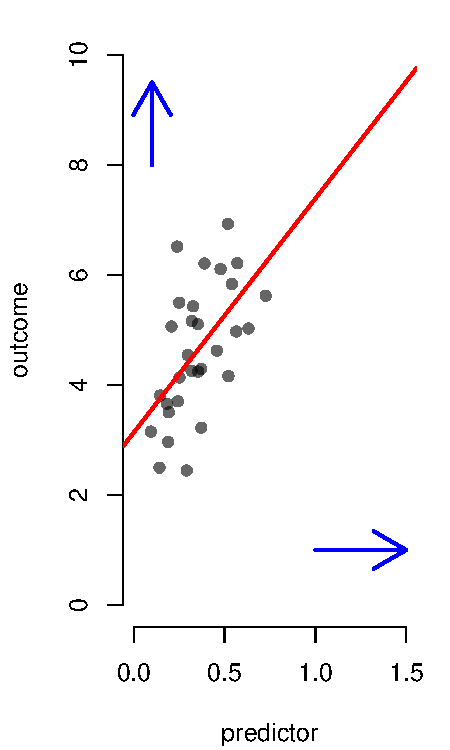
\includegraphics[height = 0.8\textheight]{linear_regression.pdf}
\end{column}
\end{columns}
    % [IMAGE LEFT: Linear Regression, + arrows for two types of extrapolation] 
  
\end{frame} 

\begin{frame}{What to do instead: Asymptotically Motivated Model}
\begin{columns}
\begin{column}{0.3\textwidth}
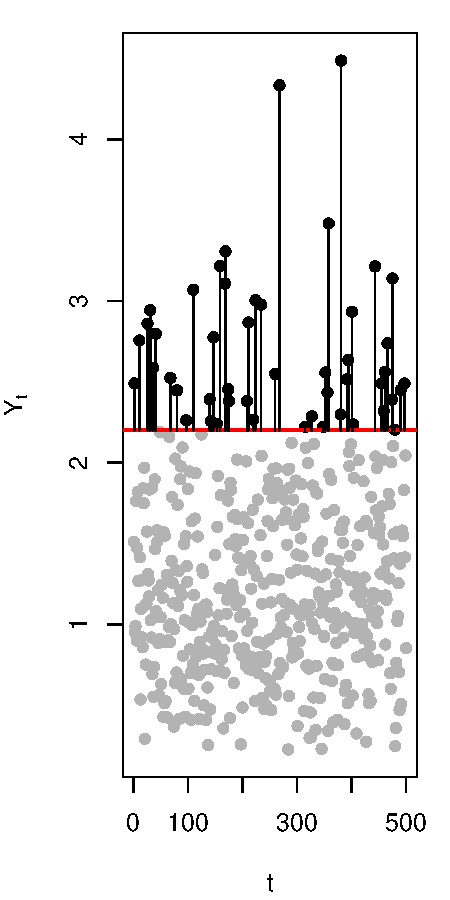
\includegraphics[width = \textwidth]{threshold_exceedances.pdf}
\end{column}
\begin{column}{0.7\textwidth}
\begin{itemize}
    \item If we want to model big values then consider only big values. \\
    \item []
    \item Define `big' as exceedances of some high threshold $u$. \\
    \item []
    \item In the limit as $u \rightarrow \infty$ then the distribution of the suitably rescaled threshold excesses converges to a single probability distribution, \textbf{regardless of the initial distribution}. \\
    \item []
    \item Extreme Value Theory tells us that this is the \textbf{Generalised Pareto Distribution}. 
\end{itemize}
\end{column}
\end{columns}
\end{frame}  

\begin{frame}{The Generalised Pareto Distribution}   
\begin{columns}
\begin{column}{0.5\textwidth}
\vspace{3em}
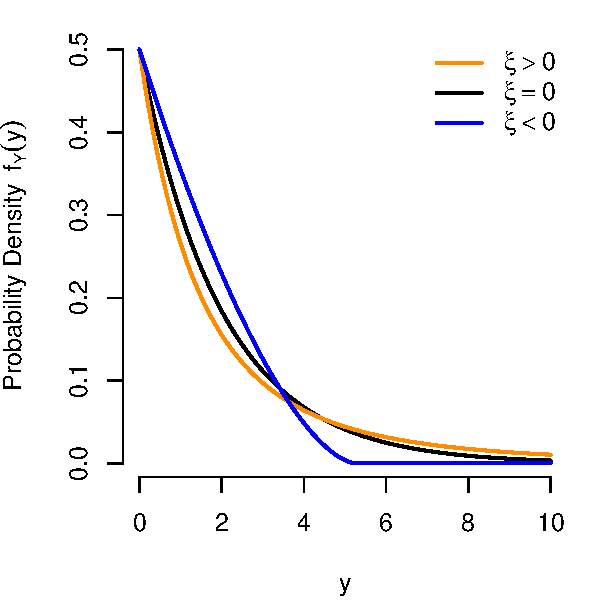
\includegraphics[width = \textwidth]{gpd_densities.pdf}
\end{column}
\begin{column}{0.5\textwidth}
\begin{itemize}
    \item $\xi = 0$: Exponential distribution $\iff$ GR Law 
    \item [] 
    \item $\xi > 0$: Pareto
    distribution $\iff$ Power Law 
    \item [] 
    \item $\xi < 0$: Finite upper endpoint, similar to exponential taper model. 
\end{itemize}
\end{column}
\end{columns}
\end{frame}

\begin{frame}{The Generalised Pareto Distribution}
\textbf{Distribution function: }

For GPD$(\sigma_u,\xi)$ exceedances of $u$
\[
F(y)= 1-\left[1+\xi\frac{y-u}{\sigma_u}\right]_+^{-1/\xi}\mbox{ for }y>u
\]
where $\sigma_u>0$ and  $x_+=\max(x,0)$.

\vspace{2em}
\textbf{Threshold stability property:} 

If GPD($\sigma_u$, $\xi$) above $u$ then for any $v>u$
\[
Y - v \mid Y > v \ \sim \  \mbox{GPD}(\sigma_u+\xi(v-u), \ \xi) \ = \  \text{GPD}(\sigma_v,\ \xi.)
\]
\end{frame}

\begin{frame}{Applying EVT to finite samples}
\begin{itemize}
    \item Apply this tractable asymptotic model at finite levels. 
    \item []
    \item Using assumptions to buy certainty:
    \begin{itemize}
        \item central limit theorem 
        \item elastic thin sheet of infinite extent
    \end{itemize} 
    \item []
    \item Not a spherical chicken in a vacuum, requires only very light assumptions on the original distribution. 
    \item []
    \item Extends to non-i.i.d. data by having threshold and parameters as a function of time or covariates.

\end{itemize}
\end{frame}

\begin{frame}{Applications of Extreme Value Theory: Natural Hazards}
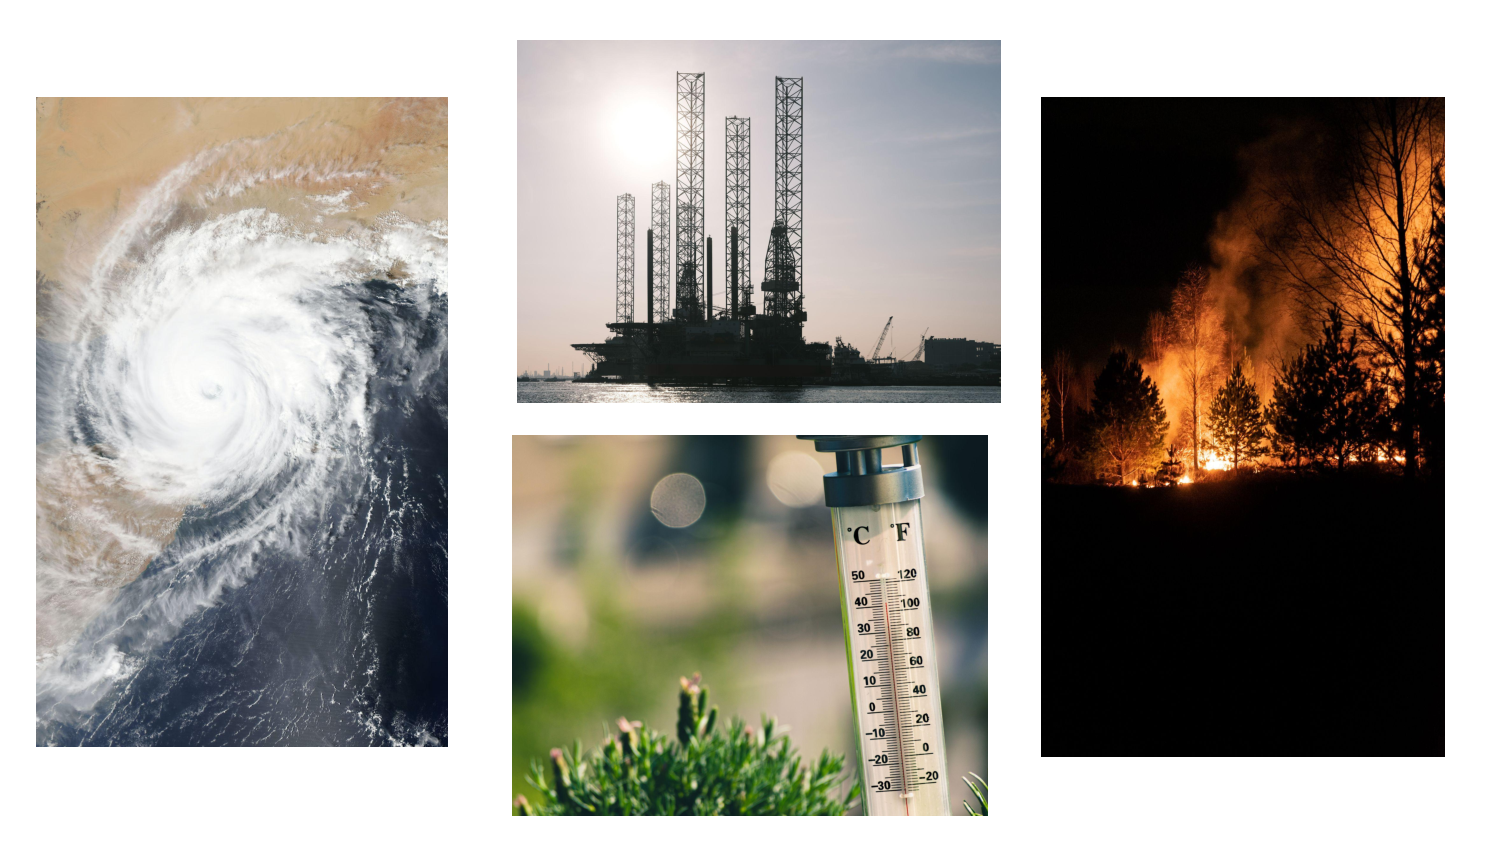
\includegraphics[page=1, width=\textwidth]{extremes_applications.pdf}
\end{frame}

\begin{frame}{Applications of Extreme Value Theory: Elsewhere}
\includegraphics[page=2, width=\textwidth]{extremes_applications.pdf}
\end{frame}


\begin{frame}{Extreme Value Theory: Summary}
\begin{itemize}
    \item EVT is a mathematically justified means of extrapolation.
    \item []
    \item Extreme value models are used as standard across many other disciplines to reflect uncertainty in the tail shape as well as its scale.
    \item []
    \item Many intrinsic parallels between EVT and seismicity models:
    \begin{itemize}
        \item threshold selection $\iff$ magnitude of completion;
        \item modelling conditional on being sufficiently large;
        \item GPD $\iff$ power law, Gutenberg-Richter, tapered magnitudes.
    \end{itemize}
\end{itemize}

\end{frame}

\section{What can small events tell us about large ones?}


\begin{frame}{Groningen Earthquake Catalogue}
  \begin{columns}
  \begin{column}{0.6\textwidth}
      \textbf{Recording:}
    \begin{itemize}
        \item Time changing measurement process; more sensors and improved sensitivity.
        \item Earthquakes missing-not-at-random.
        \item Rounding to $0.1~M_L$.
    \end{itemize}
    \vspace{2em}
   \textbf{Magnitude of completion $m_c(t)$:}
    \begin{itemize}
    \item Smallest magnitude at which earthquake in region is certain to be recorded
    \end{itemize}
    \vspace{1em}
    \small{Work in 'event time' and back-transform}
  \end{column}
  \begin{column}{0.4\textwidth}
  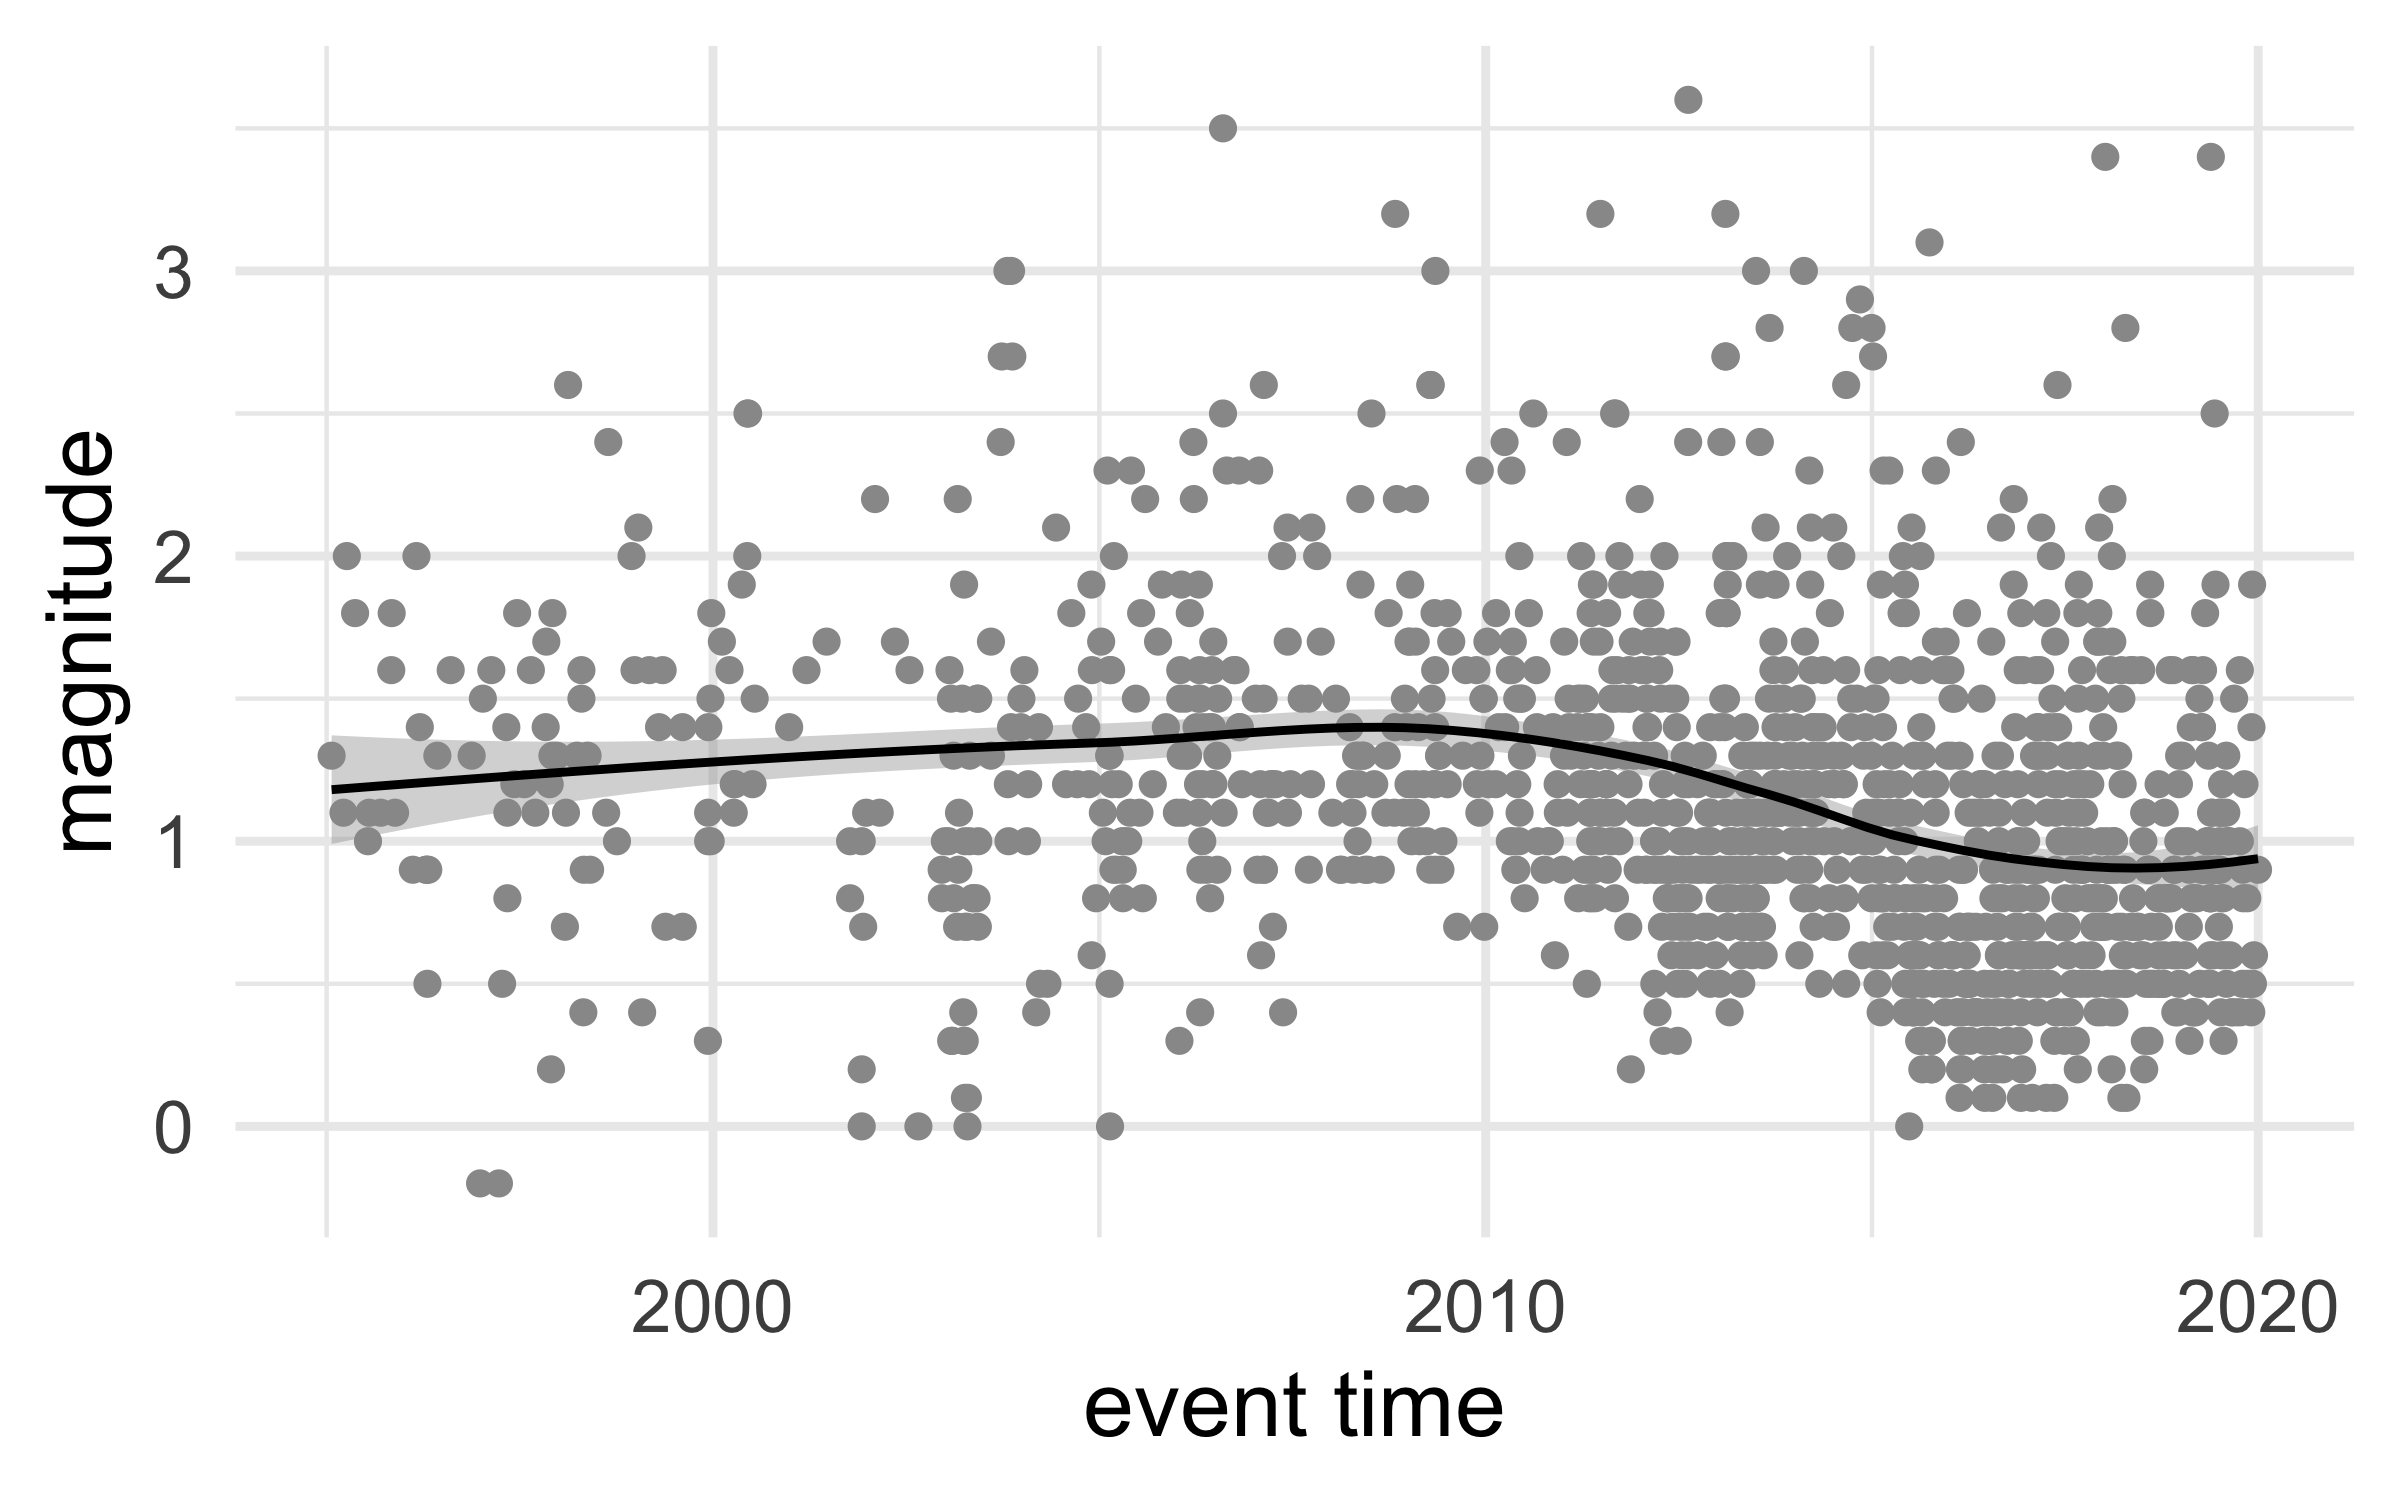
\includegraphics[width = \textwidth]{groningen_catalogue_natural.png}
  \\
  \vspace{2em}
  \includegraphics[width = \textwidth]{groningen_catalogue_index.png}
  \end{column}
  \end{columns}  
\end{frame}

\begin{frame}{Aims of Inference}
    \begin{enumerate}
        \item Automate estimation of a time-varying $m_c$.
        \item Estimate and lower $m_c(t)$ from current standard
        \item []
        \begin{itemize}
            \item $m_c= 1.45~M_L$, after 2014 reduced to $m_c = 0.95~M_L$.
        \end{itemize}
        \item Use additional information to \textbf{estimate the upper tail of magnitude distribution} - high quantiles and $m_{\text{max}}$. 
        \item Test consistency with Gutenberg Richter Law.
        \item Develop method to handle:
    \begin{itemize}
        \item trade off in quality of fit vs inference uncertainty
        \item rounding
        \item non-stationarity
        \item informative missingness
        \end{itemize}
    \end{enumerate}
\end{frame}


\begin{frame}{Existing Methods \& Limitations}
\textbf{Threshold Selection}
\begin{itemize}
    \item Parameter stability plots
    \item Linearity of magnitude frequency relationship
    \item PP and QQ plots 
    \item []
    \item Summaries such as Anderson-Darling
    \item Rolling quantile
\end{itemize}

\textbf{Inference}
\begin{itemize}
    \item Seismic models underestimate epistemic uncertainty
    \item Roounding and Censoring
\end{itemize}
\end{frame}

\begin{frame}{New Strategy: Model Structure}
    \begin{itemize}
\item Data $(t_i,x_i): i=1,\ldots ,n$
\item $x_i$ rounded magnitudes, rounding to nearest $2\delta$
\item $y_i$ true magnitudes
\item $y_i\in (x_i-\delta, x_i+\delta]$
\item event index $\tau$
\item threshold (unknown) $v(\tau)\equiv (v_1, \ldots ,v_n)$ 
\item $Y_i-u\mid Y_i>u \sim \mbox{GPD}(\sigma_u,\xi)$ for $u<\min(v_1, \ldots ,v_n)$
\end{itemize}
\pause
\textbf{Three cases:}
\begin{itemize}
\item $x_i>v_i+\delta \implies y_i>v_i$
\item $x_i<v_i-\delta \implies y_i<v_i$
\item $\mid x_i-v_i\mid<\delta \implies y_i>v_i$  with probability $w_i$
\end{itemize}
\end{frame}

\begin{frame}{Likelihood Based Inference}
For rounded GPD data and a given threshold  $v(\tau)$:

\begin{align*} 
    \ell(\bm{\theta} | \bm{x}, \bm{v})
    &= \sum_{i = 1}^{n} w_i \log \Pr(X_i = x_i | Y_i > v_i, \bm{\theta}) \nonumber\\
    & = \sum_{i = 1}^{n} w_i \log \Pr( \max(v_i, x_i - \delta) < Y_i < x_i + \delta | \bm{\theta}) %\label{eqn:rounded_gpd_likelihood}
%    \\
%    & = \sum_{i = 1}^{n} 
%  w_i
%    \log\left[ 
%         F(x_i + \delta - v_i; \sigma_{v_i}, \xi) - F(\max(v_i, x_i - \delta) - v_i; \sigma_{v_i}, \xi)
%        \right], \nonumber
\end{align*}
where 
    \[
    w_i =  \frac{\Pr( \max(v_i, x_i - \delta) < Y_i < x_i + \delta | \bm{\theta})}{\Pr( x_i - \delta < Y_i < x_i + \delta | \bm{\theta})} . \]
 
\vspace{1em}  
\pause
\textbf{Issue:} Changing sample size rules out standard model comparison
\end{frame}

\begin{frame}{Measuring Fit: Metric definitions}
Calculated on standard exponential scale (threshold invariance and PIT).

\begin{align*}
    d_0=d(q,1) = \frac{1}{m} \sum_{j=1}^{m} |-\log(1-p_j) - Q(p_j)|
\end{align*}
%and 
\begin{align*}
    d_0=d(q,2) = \frac{1}{m} \sum_{j=1}^{m} (-\log(1-p_j) - Q(p_j))^2.
\end{align*}
%
\begin{itemize}
\item Sequence of probabilities $p_i=i/(m+1)$\\
\item $Q$ is empirical quantile function
\item PP methods- much less effective
\end{itemize}

\end{frame}

\begin{frame}{New Threshold Selection Strategy}%the content in the frame will be displayed as the title of the page

\underline{\textbf{For given threshold choice for $v(\tau)$:}}
\begin{itemize}
\item Assess fit using QQ or PP plot
\item Use metric to summarise difference between model and empirical - $d_0$
\item Parametric bootstrapped replicates of $X$ $\implies \hat{\theta}_{GPD} \implies Y$ 
\begin{itemize}
\item Sample size varies (due to rounding)
\item Take expectation over latent $Y$ and $\hat{\theta}_{GPD}$ variables
\end{itemize}
\end{itemize}
$\implies$ Output
$d=E_{Y, \hat{\theta}_{GPD}\mid x,v(\tau)}(d_0)$  (subject to Monte Carlo noise)

\pause

\underline{\textbf{Automatic selection of $v(\tau)$:}}
\begin{itemize}
\item Parametric $v(\tau)$ with parameters $\theta_v$
\item Minimise $d$ over $\theta_v$
\item Minimise using grid-search for low dimensional $\theta_v$
\item Minimise using Bayesian optimisation methods for higher dimensional $\theta_v$
\end{itemize}
\end{frame}

\begin{frame}{Parametric Threshold Models}
\textbf{Flat:} $\theta_v=(v)$

$$v(\tau)= v.$$  

\textbf{Stepped:} $\theta_v=(v_L, v_R, \tau^*)$
\[
v(\tau)=\left\{ 
\begin{array}{ll}
v_L & \mbox{ if }\tau\le \tau^*\\
v_R & \mbox{ if } \tau > \tau^*\\
\end{array}
\right.
\]

\textbf{Sigmoid:} $\theta_v=(v_L, v_R, \tau^*, \gamma)$

\[
v(\tau)=v_R+(v_L-v_R)\Phi\left(\frac{\tau^*-\tau}{\gamma}\right)
\]
\end{frame}

\section{Threshold Selection on Simulated Catalogues}

\begin{frame}{Simulated Catalogue Structure}
\textbf{Censoring methods:} (i) hard and (ii) phased.
%
In phased censoring the detection probability of each event is 
\[
\alpha(y_i,v_i) = \exp(-\lambda[v_i-y_i]_+), \mbox{ where } \lambda>0.
\]
%
\begin{figure}[hbt!]
    \centering
    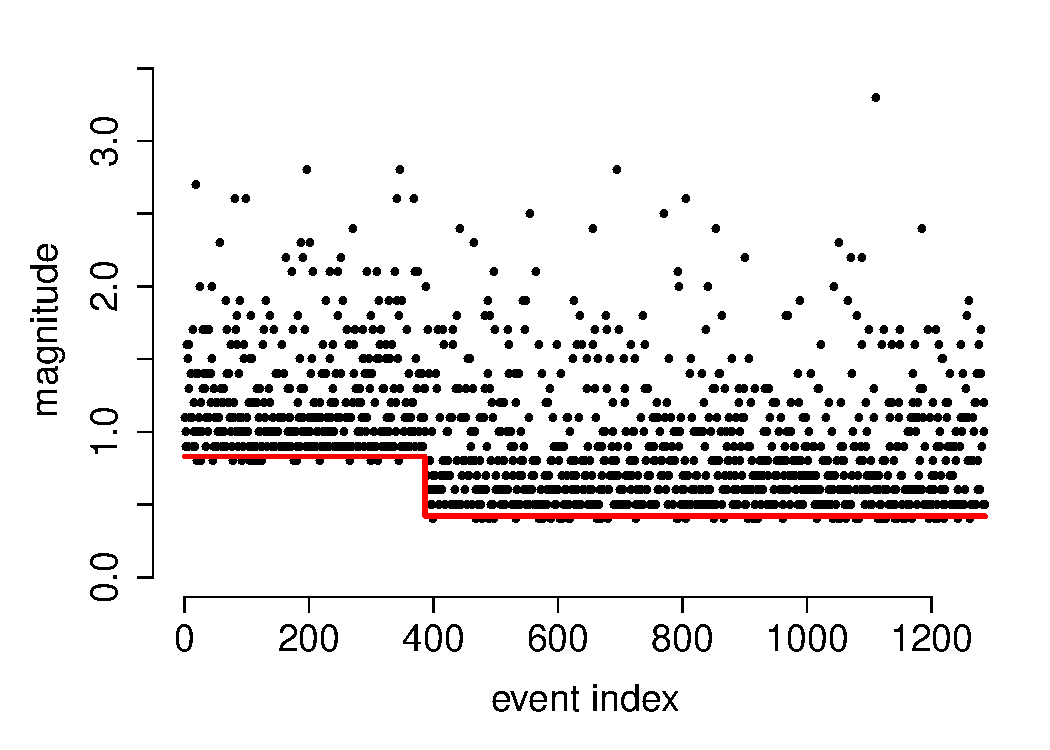
\includegraphics[width = 0.4\textwidth]{images/step_threshold_sim/example_cat_stepped_hard.pdf}
    \qquad
    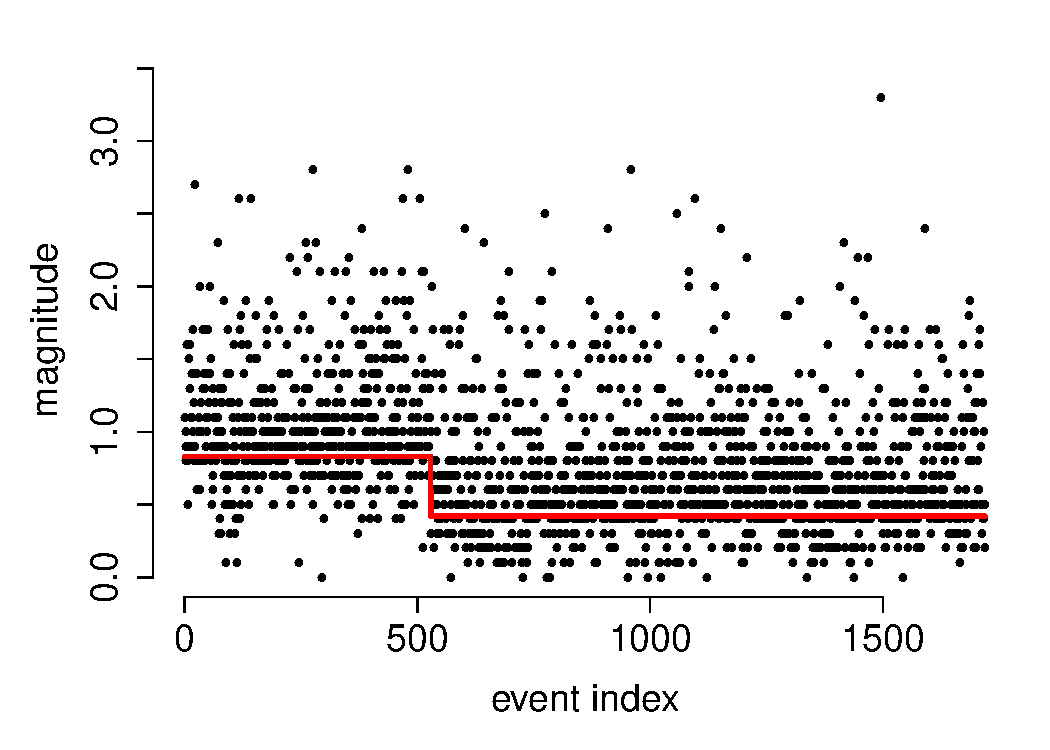
\includegraphics[width = 0.4\textwidth]{images/step_threshold_sim/example_cat_stepped_phased.pdf}
    \caption{Example simulated catalogues with hard censoring [left] and phased censoring [right] for stepped thresholds of $(v_L,v_R)$ = (0.83,0.42), shown as a red line,  and phasing parameter $\lambda = 7$.}
    \label{fig:stepped_cat_examples}
\end{figure}    
\end{frame}

\begin{frame}{Flat Threshold, Hard Censoring:  Single Catalogue}
    \begin{figure}
    \centering
    \includegraphics[width = 0.45\textwidth, page = 2]{images/flat_threshold_sim/qq_metrics.pdf}
    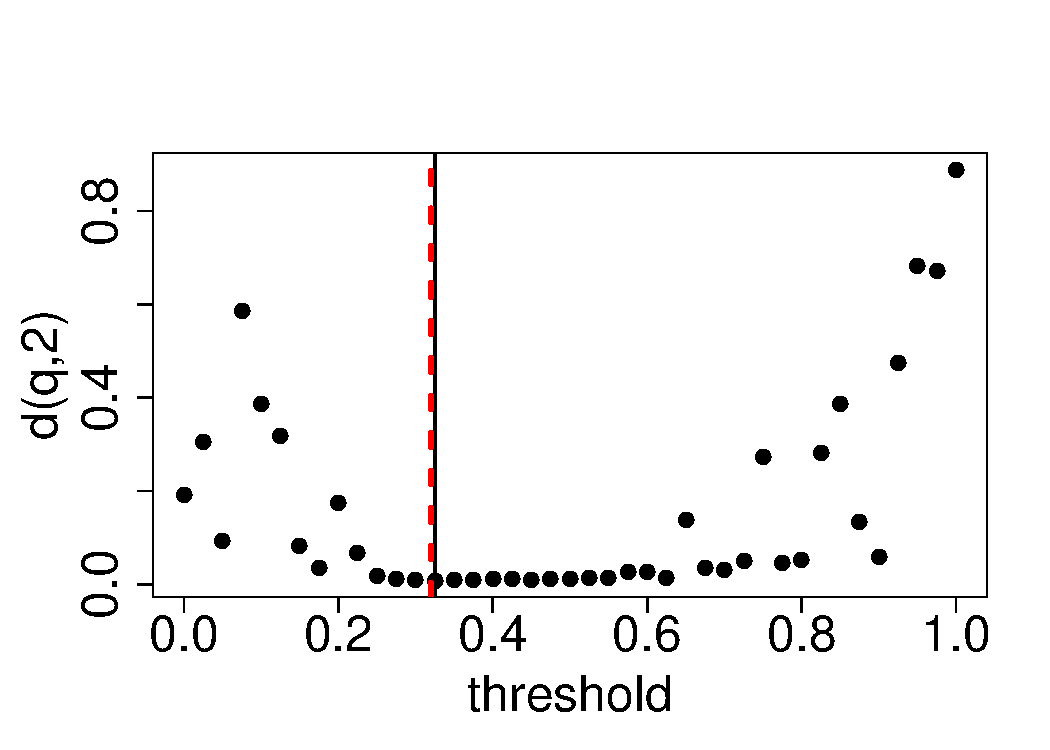
\includegraphics[width = 0.45\textwidth, page = 1]{images/flat_threshold_sim/qq_metrics.pdf} 
%    \\
%    \includegraphics[width = 0.35\textwidth, page = 2]{figures/flat_threshold_sim/pp_metrics.pdf}
%    \includegraphics[width = 0.35\textwidth, page = 1]{figures/flat_threshold_sim/pp_metrics.pdf} %\\
    \caption{Flat threshold selection on a simulated catalogue. Top row: expected mean absolute [left] and expected mean squared [right] QQ-distances against threshold value.  Selected and true thresholds are indicated by solid black and dashed red lines.}
    \label{fig:flat_threhsold_sim}
\end{figure} 
\end{frame}

%%%
\begin{frame}{Flat Threshold, Hard Censoring: Replicate Results}
\begin{figure}
    \centering
    %
    \includegraphics[width = 0.45 \textwidth, page = 1]{images/flat_threshold_sim/selected_threshold_summary_individual.pdf}
    \qquad
    \includegraphics[width = 0.45\textwidth, page = 2]{images/flat_threshold_sim/selected_threshold_summary_individual.pdf}
    %% !!! NB: PP selections are in pages 3 and 4 - uncomment to add !!!
    %\includegraphics[width = 0.4 \textwidth, page = 3]{figures/flat_threshold_sim/selected_threshold_summary_individual.pdf}
    %\qquad
    %\includegraphics[width = 0.4\textwidth, page = 4]{figures/flat_threshold_sim/selected_threshold_summary_individual.pdf}
    %
    \caption{Sampling distribution of threshold selection methods for quantile-based metrics over 500 simulated catalogues with constant threshold and hard censoring. The true threshold is shown by a dashed red line and the root mean squared error (RMSE) for each method is given in plot titles.}
    %
    \label{fig:flat_threshold_selection_summary}
\end{figure} 
Focus now only the absolute error QQ metric
\end{frame}
%%%

\begin{frame}{Comparison of Hard and Phased Censoring}
    \begin{figure}[hbt]
    \centering
    \includegraphics[width = 0.9\textwidth, page = 2]{images/changepoint_sim_hard/selection_errors_II_changepoint_hard.pdf}\\
     \includegraphics[width = 0.9\textwidth, page = 2]{images/changepoint_sim_phased/selection_errors_II_changepoint_phased.pdf} 
    \caption{Marginal sampling distributions of errors in the selected values of $v^{(1)}$ (left),  $v^{(2)}$ (center) and $\tau^*$ (right) for 500 simulated catalogues with change-point type thresholds and hard (top row) or phased (bottom row) censoring. }
    \label{fig:changepoint_errors}
\end{figure}
\end{frame}

\section{Application to Groningen Catalogue}

\begin{frame}{Application to Groningen catalogue}
%%% 

\textbf{Comparing GPD vs Gutenberg-Richter above conservative threshold:}
\begin{columns}
\begin{column}{0.55\textwidth}
\begin{itemize}
\item Conservative threshold: $v_C=1.45 M_L$
\item 311 exceedances
\item $\hat{\xi}=-0.018$ 
\item (if rounding ignored $\hat{\xi}=-0.027$)
\item Bootstrap $95\%$ CI:   $(-0.147; 0.086)$
\item Can't rule out Gutenberg-Richter law (Exponential tail)
\end{itemize}
\end{column}
\begin{column}{0.45\textwidth}
\\
\vspace{3em}
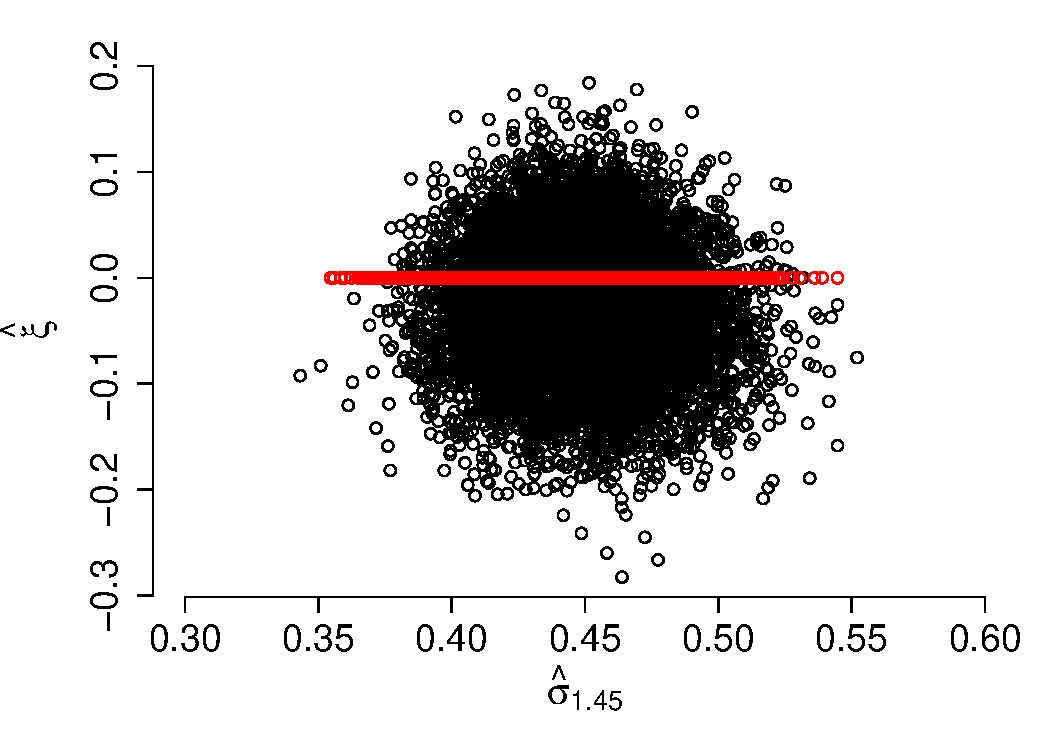
\includegraphics[width = 0.8\textwidth]{groningen_application/motiving_GPD_over_exponential/groningen_conservative_boot_mles.pdf}
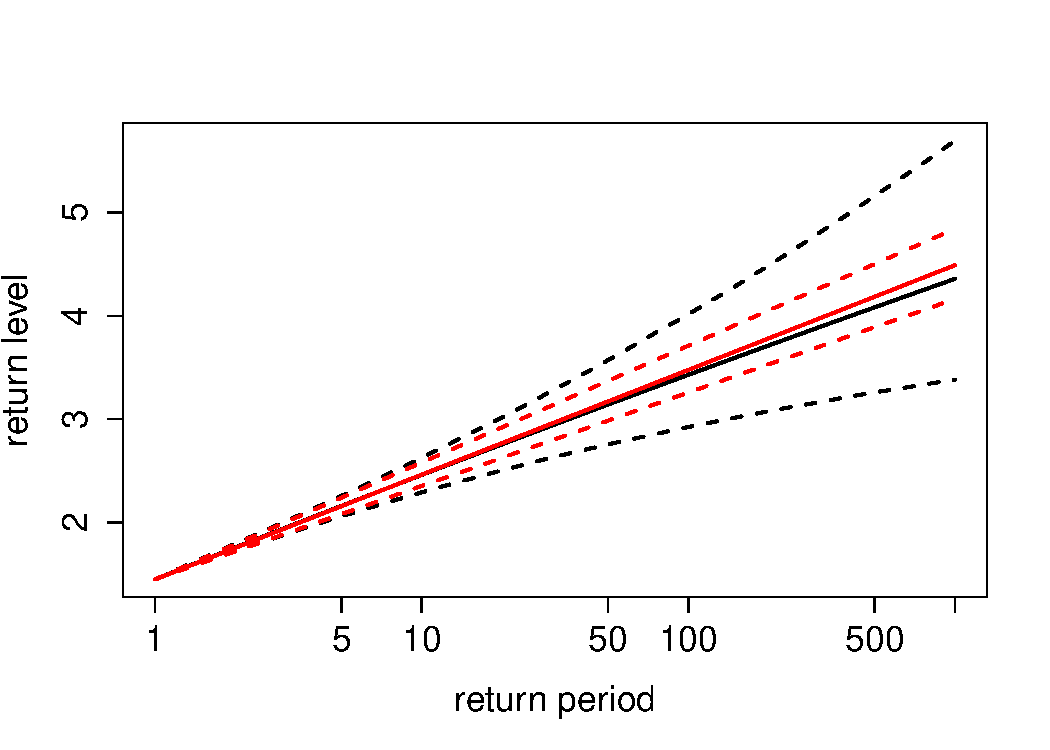
\includegraphics[width = 0.8\textwidth]{groningen_application/motiving_GPD_over_exponential/return_levels_conservative.pdf}
\end{column}
\end{columns}
\end{frame} 

\begin{frame}{GPD fits well above $v_C$}
\begin{figure}
    \centering
%    \includegraphics[width = 0.4\textwidth, page = 1]{figures/groningen_application/motivating_GPD_over_exponential/groningen_conservative_mod_PP_QQ.pdf}
%    \qquad
    \includegraphics[width = 0.5\textwidth, page = 2]{groningen_application/motiving_GPD_over_exponential/groningen_conservative_mod_PP_QQ.pdf}
    \caption{QQ plot for Groningen magnitudes exceeding 1.45$\text{M}_{\text{L}}$ under the GPD model. Grey regions show $95\%$ tolerance intervals while vertical lines show $95\%$ confidence intervals on sample probabilities / quantiles. All confidence intervals overlap with the associated tolerance intervals.  }
  %  \label{fig:groningen_mod_pp_qq_above_145}
\end{figure}
\end{frame}


\begin{frame}{Flat Threshold Selection}
    \begin{figure}
    \centering
     \qquad
        \includegraphics[width = 0.4\textwidth]{images/motivating_data/groningen_catalogue_index.png} 
    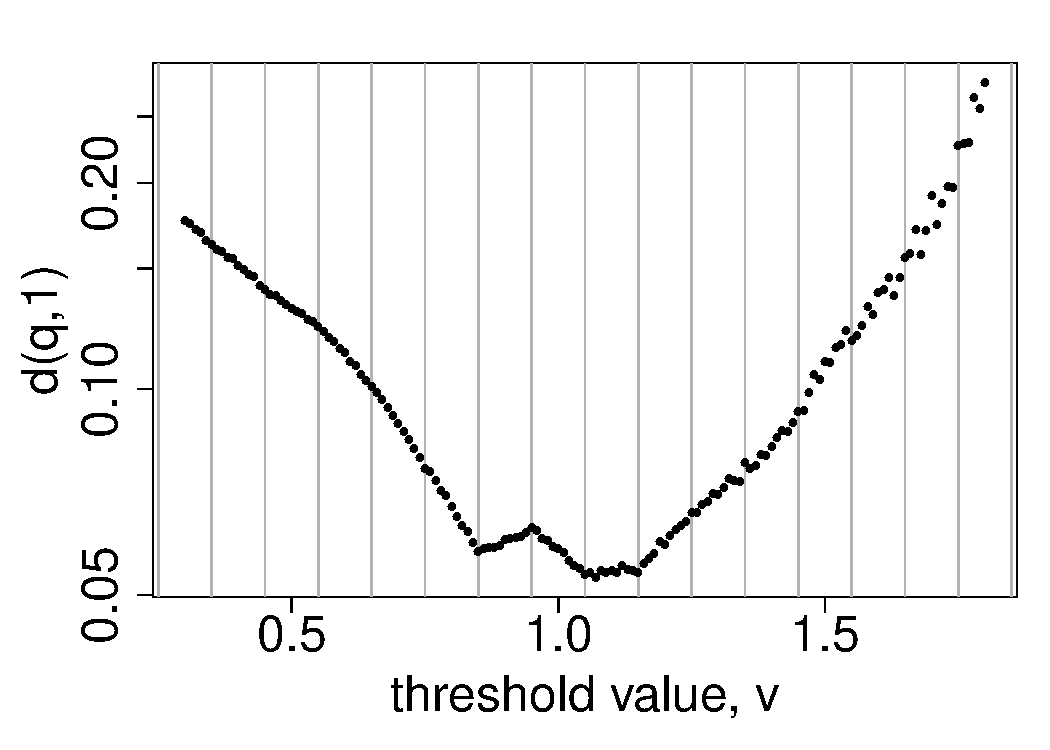
\includegraphics[width = 0.45\textwidth]{images/groningen_application/flat_threshold_selection/groningen_flat_metric_values.pdf}
%    \qquad
%    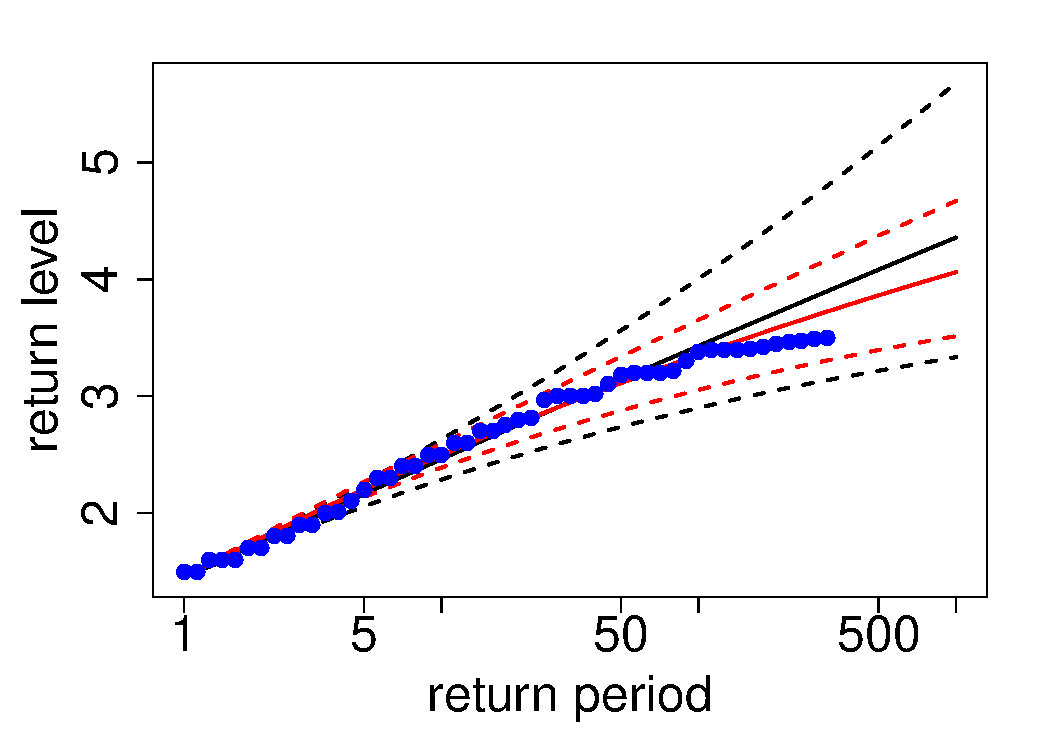
\includegraphics[width = 0.45\textwidth]{figures/groningen_application/flat_threshold_selection/groningen_flat_selected_return_levels.pdf}
    \caption{[Left] Data,  [Right] Grid search to minimise $d(q,1)$ over threshold values flat threshold. Metric values are shown on log-scale and vertical lines mark the edges of magnitude rounding intervals}
    \label{fig:groningen_flat_selection_metrics_values}
\end{figure}
\begin{itemize}
\item $v_C=1.45$ is a poor choice 
\item Two minima of interest
\end{itemize}
\end{frame}


\begin{frame}{Sigmoid Threshold Selection}
\begin{figure}
    \centering
    %%
    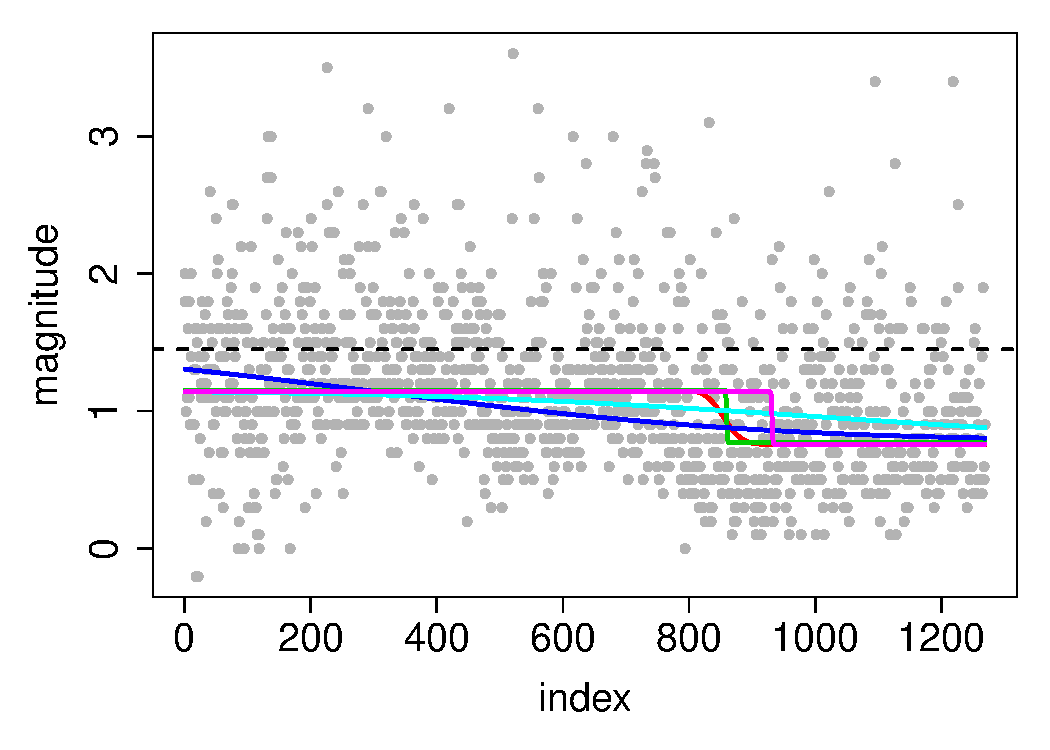
\includegraphics[width = 0.32\textwidth]{images/groningen_application/sigmoid_threshold_selection/BO_selected_thresholds.pdf} 
    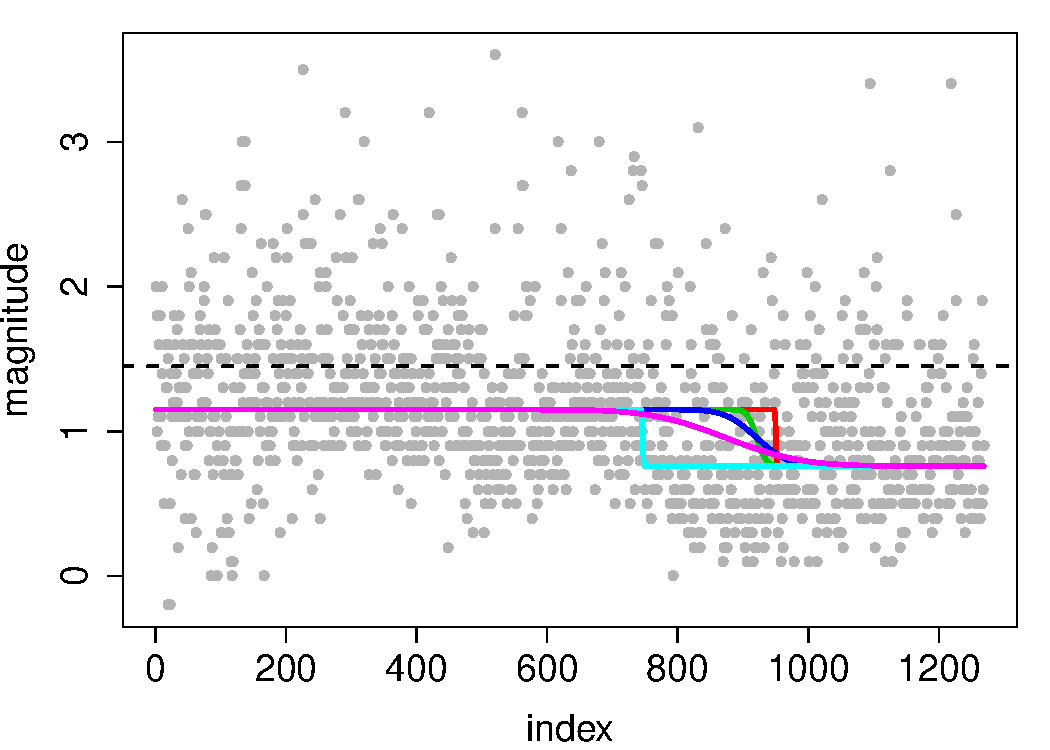
\includegraphics[width = 0.32\textwidth]{images/groningen_application/sigmoid_threshold_selection/BO_selected_thresholds_restricted.pdf}
    %%
    \includegraphics[width = 0.32\textwidth, page = 2]{images/groningen_application/sigmoid_threshold_selection/BO_selected_thresholds_restricted.pdf}
    %%
    \caption{ Selected sigmoid thresholds using Bayesian optimisation. [left] Optimising over all thresholds parameters. [centre, right] Optimising over $(\tau^*, \gamma)$ and fixing $(v_{L}, v_{R})$ = $(1.15,0.76)$ on index- (centre) and natural- (right) timescales. Dates: 
     (A) network development begins, (B) first additional sensors activated, (C) upgrade complete.}
    %%
    \label{fig:groningen_selected_sigmoid_thresholds}
\end{figure}
\vspace{-1em}
\textbf{Data used above thresholds and value of $d\times 1000$:}
\begin{itemize}
\item Conservative choice:  $n_v=311$, $d= 91$
\item Best flat: $n_v=627$, $d=54$
\item Best sigmoid: $n_v=702$, $d=41$
\end{itemize}
\end{frame}


\begin{frame}{Benefits of lower threshold}
\begin{itemize}
\item Lowered $m_c(\tau) \implies$ more data to use
\item Better parameter inference
\item $\hat{\xi}=-0.069$ $95\%$ CI $(-0.144, -0.008)$
\item Excludes zero: weak evidence against Gutenberg-Richter law
\end{itemize}


\begin{figure}
    \centering
    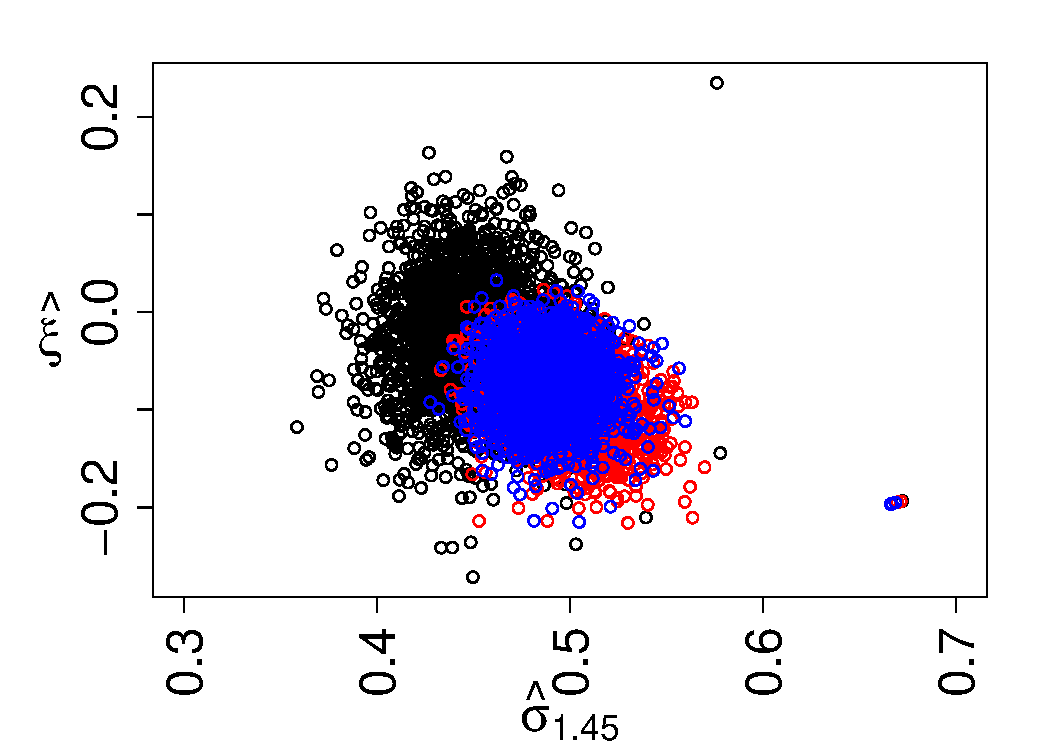
\includegraphics[width = 0.45\textwidth]{images/groningen_application/sigmoid_threshold_selection/parameter_comparison_cons_flat_sigmoid.pdf}
    \qquad
    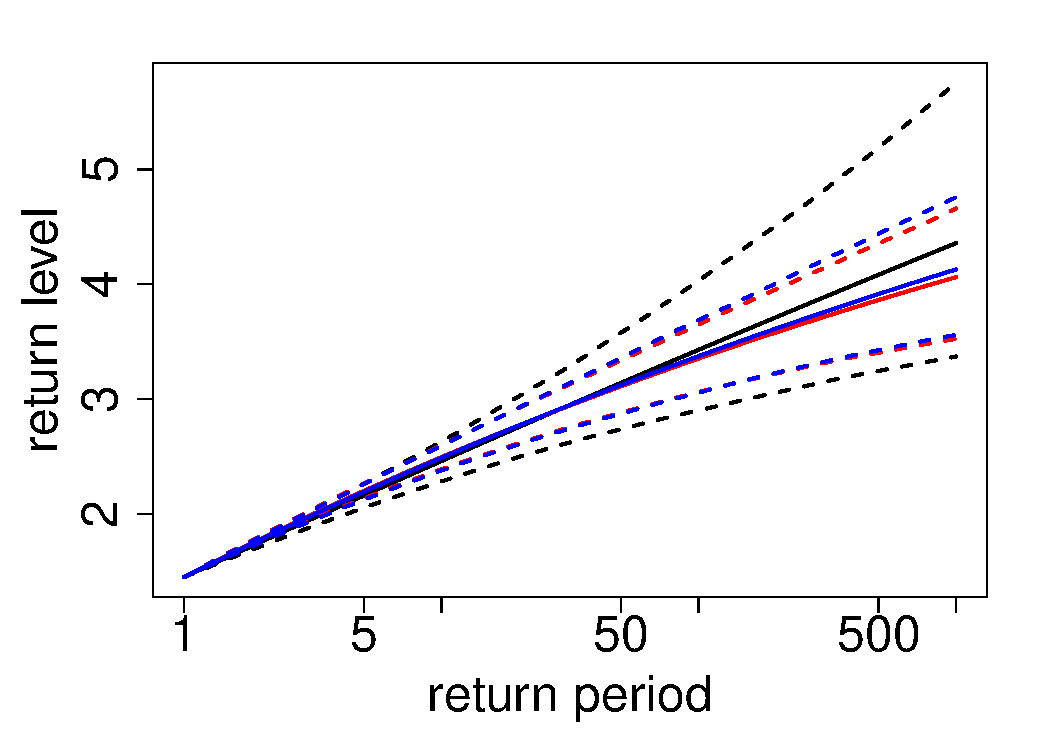
\includegraphics[width = 0.45\textwidth]{images/groningen_application/sigmoid_threshold_selection/return_level_comparison_cons_flat_sigmoid.pdf}
    \caption{Bootstrap GPD parameter estimates based on exceedances of the conservative (black), \textcolor{red}{flat} and \textcolor{blue}{sigmoid} thresholds [left]. Estimated return levels in $\text{M}_{\text{L}}$ and $95\%$ confidence intervals for magnitudes exceeding $1.45\text{M}_{\text{L}}$ [right]. }
    \label{fig:groningen_threshold_comparison}
\end{figure}
\end{frame}

\begin{frame}{Summary}
    \begin{enumerate}
        \item The Generalised Pareto Distribution unifies magnitude-frequency relationships, better representing epistemic uncertainty.
        \item []
        \item Including small magnitude events is cost effective and informative. 
        \item []
        \item Using a time varying threshold gives evidence of sub-exponential decay. 
        \item []
        \item Magnitude-Frequency relationship is described as we approach $M_{\text{max}}$, while properly accounting for uncertainties.
    \end{enumerate}
\end{frame}

\begin{frame}{Further Work}
\begin{columns}
\begin{column}{0.6\textwidth}
    \begin{itemize}
        \item \textbf{Does choice of measurement scale matter?} \checkmark \\ Hartog and Bierman investigated robustness to choice of measurement scale. 
        \item []
        \item \textbf{Are Exponential margins optimal?} \\ Murphy simulation study shows smaller changes can be better. 
        \item []
        \item \textbf{Can we do this without aggregating over space?} \checkmark  \\ Murphy extending to spatial threshold selection. 
    \end{itemize}
\end{column}
\begin{column}{0.4\textwidth}
\vspace{3em} 
 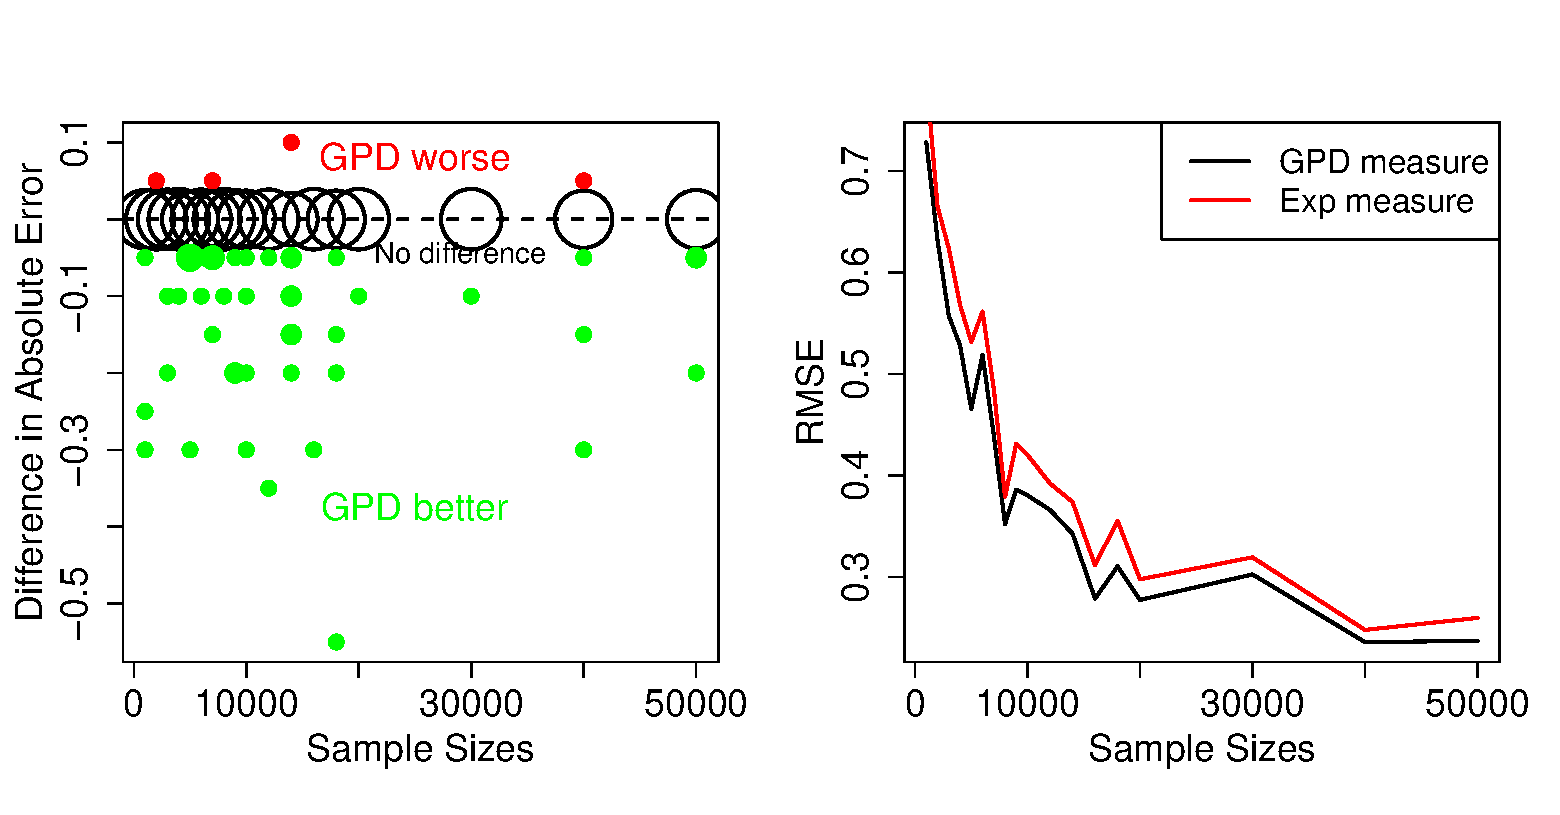
\includegraphics[width = \textwidth]{CaseStudy.pdf} \\
   \vspace{2em} 
    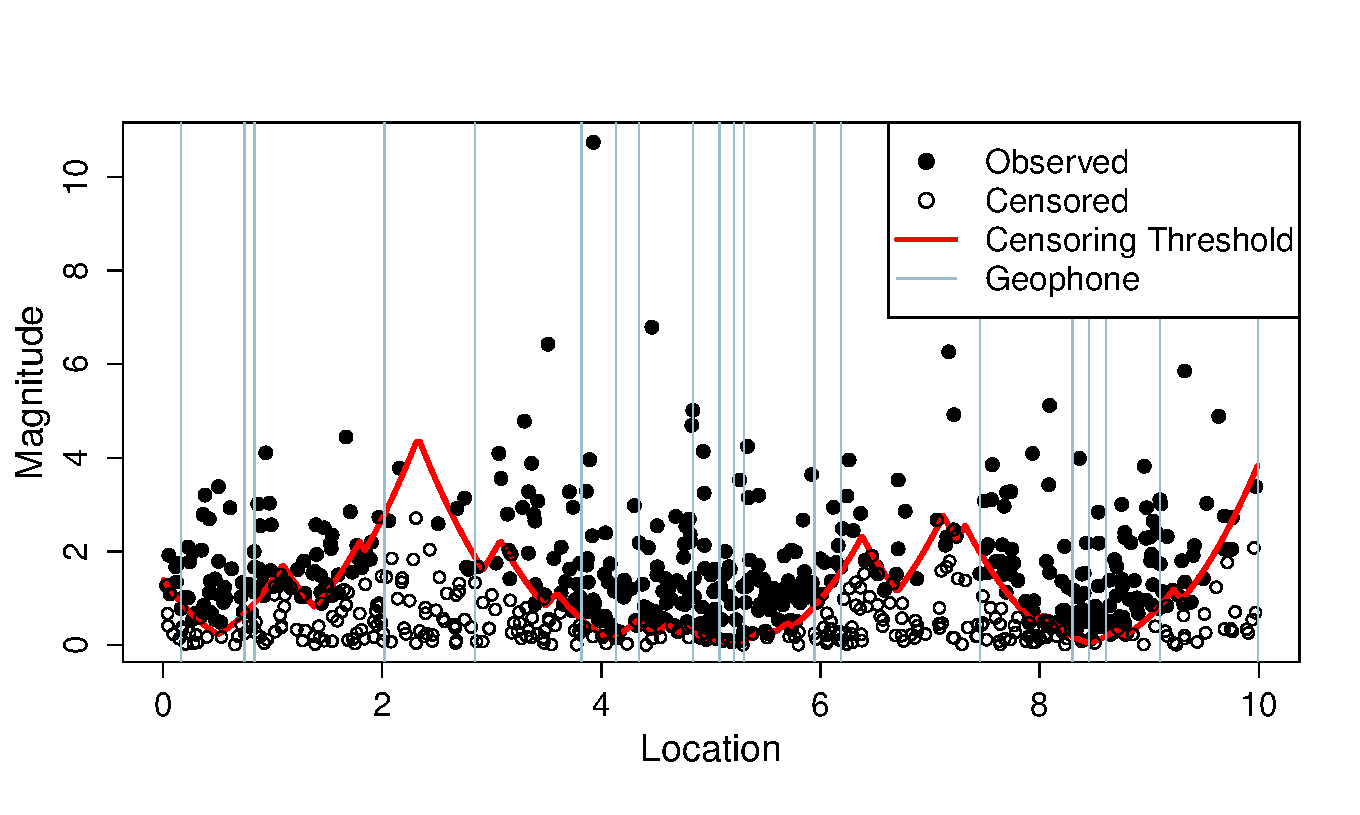
\includegraphics[width =  \textwidth]{Spatial_censoring_1D.3.pdf}
\end{column}
\end{columns}
\end{frame}


\begin{frame}{Further, Further Work}
    \begin{itemize}
        \item \textbf{Can we include stress-dependent magnitudes?} \\ More challenging because requires separation of effects. 
        \item []
        \item \textbf{How does this impact prediction?} \\ Combining models and propagating uncertainty about earthquake number, rate and size. 
        \item []
        \item \textbf{Can we demonstate effectiveness  in other settings?} \\ Also useful in more general EVT settings, improved detection common. Suggested applications welcome.
    \end{itemize}
\end{frame}

\section{Thank you. Any Questions?}

\appendix

\begin{frame}{Threshold Selection Paper}

Varty, Z., Tawn, J. A., Atkinson, P. M., \& Bierman, S. (2021). Inference for extreme earthquake magnitudes accounting for a time-varying measurement process. \href{https://arxiv.org/abs/2102.00884}{arXiv preprint arXiv:2102.00884.}

\end{frame}


\begin{frame}
\frametitle{Lancaster’s EVT Impact}
{\bf Univariate Extremes}

\begin{itemize}

\item Optimising the height of all coastal flood protection schemes in the UK, saving \pounds 200-300M over 13 years. \href{https://rss.onlinelibrary.wiley.com/doi/abs/10.2307/2347619}{[link to paper]}

\item Identified the likely cause of the sinking in 1980 of the MV Derbyshire for the \pounds 11M High Court Formal Investigation.
\href{https://rss.onlinelibrary.wiley.com/doi/full/10.1111/1467-9876.00408}{[link to paper]}

\item {\it Calculated worldwide design standards for bulk carrier hold strength, impacted on the design of 6000 carriers - resulting in many saved ships/lives} 
\href{https://link.springer.com/article/10.1023/A:1016544112941}{[link to paper]}
\end{itemize}
\end{frame} 

\begin{frame}

\frametitle{ Lancaster’s EVT Impact}

{\bf Multivariate/Spatial Extremes}

\begin{itemize}

\item

{\it Optimise the structural integrity of over 8\% of worldwide offshore oil and gas facilities, saving \pounds 80M} \href{https://www.sciencedirect.com/science/article/pii/S002980181930784X}{[link to paper]}

\item

Developing the widespread flooding scenarios for the UK Government's National Risk Assessment for river + coastal \href{https://www.sciencedirect.com/science/article/pii/S0029801817305048}{[link to paper]} 


\item

Developing spatial flood risk methods for the UK Government's 2016 National Flood Resilience Review:

{\it e.g., What is probability of a 1 in 100 year event at a site occurring anywhere in UK in a year?} \href{https://www.sciencedirect.com/science/article/pii/S2211675317302786}{[link to paper]}
\end{itemize}
\end{frame} 

\begin{frame}
\frametitle{International EVT Impact}
\begin{itemize}
\item Netherlands: Coastal flooding \href{https://www.sciencedirect.com/science/article/pii/S0378383913002159}{[paper link]}
\item []
\item US: Hurricanes \href{https://agupubs.onlinelibrary.wiley.com/doi/full/10.1029/2019GL086138}{[paper link]}
\item []
\item France: Nuclear Safety \href{https://asmedigitalcollection.asme.org/ICONE/proceedings-abstract/ICONE2020/V002T08A022/1088613}{[paper link]}
\item []
\item Japan: Earthquake (Annual $M_{\text{max}}$ estimation)  \href{https://www.scirp.org/journal/paperinformation.aspx?paperid=106047}{[paper link]}
\end{itemize}
\end{frame} 

\begin{frame}
\frametitle{Non-Environmental EVT Impact}
\begin{itemize}
\item Finance: Value-at-risk, portfolio selection \href{https://www.tandfonline.com/doi/abs/10.1080/10920277.1999.10595797}{[link to paper]}
\item []
\item Sport: rankings across events/records, ultimate performances \href{https://www.tandfonline.com/doi/abs/10.1198/016214508000000698}{[link to paper]}
\item []
\item Mortality: Upper bound on Oldest Human Ages \href{https://royalsocietypublishing.org/doi/full/10.1098/rsos.202097}{[link to paper]}
\end{itemize}
\end{frame} 



\end{document}